% le caratteristiche richieste dall'università sono elencate qui: https://stem.elearning.unipd.it/mod/book/view.php?id=234&chapterid=46#modalita
% 12pt: font richiesto dall'università
% twoside: i margini interni ed esterni sono scambiati per le pagine "a sinistra" e "a destra"
% openright: i capitoli cominciano in pagine dispari ("a destra")
% extreport: supporta 12pt
\documentclass[12pt,a4paper,twoside,openright]{extreport}

\usepackage{amsmath}                            % per avere più controllo sulle equazioni 
\usepackage{amssymb}                            % For mathematical symbols and environments
\usepackage{csquotes}                           % per le citazioni
\usepackage{enumitem}                           % per avere più controllo sulle enumerazioni
%\usepackage{algorithm}
%\usepackage{algpseudocode}
\usepackage{algorithm2e}
%https://texdoc.org/serve/algorithm2e/0
\RestyleAlgo{ruled}

%% This declares a command \Comment
%% The argument will be surrounded by /* ... */
\SetKwComment{Comment}{/* }{ */}

\usepackage{hyperref}

\usepackage[
    a4paper,
    top=2cm,bottom=2cm,
    outer=2cm,inner=3cm,
    includeheadfoot
]{geometry}                                     % margini richiesti dall'università
\usepackage{graphicx}                           % per le immagini
\usepackage{icomma}                             % per separare le cifre decimali con una virgola
\usepackage{minted}                             % per il codice con la colorazione della sintassi
\usepackage[a-1a]{pdfx}                         % formato richiesto dall'università
\usepackage[output-decimal-marker={,}]{siunitx} % per le unità di misura
\usepackage{subcaption}                         % per le sottodidascalie
\usepackage{svg}                                % per inserire file SVG

\usepackage[utf8]{inputenc}
\usepackage{graphicx, animate}
\usepackage{svg}

%\usepackage[italian]{babel}
%\selectlanguage{italian}
\usepackage[english]{babel}
\selectlanguage{english}

\usepackage[backend=bibtex,style=ieee]{biblatex}
\bibliography{bibliografia}

\usepackage{fontspec}
\setmainfont{Times New Roman} % carattere richiesto dall'università

\usepackage{setspace}
\onehalfspacing % interlinea richiesta dall'università

\sloppy % per evitare che il testo in \verb finisca oltre i margini

% questi valori vengono usati nella composizione del frontespizio
\title{A Comparative Study of Optimization Techniques for the Traveling Salesman Problem}
\date{2023-2024}
\newcommand{\supervisor}{Fischetti Matteo}
\newcommand{\firstauthor}{Felline Andrea - 2090597}
\newcommand{\secondauthor}{Pietrobon Andrea  - 2087639}
%\newcommand{\assistantsupervisor}{Cognome Nome}

\begin{document}
    \pagenumbering{roman}
    \pagestyle{empty} % per le prime pagine, non mostrare il numero di pagina

    % In your document body
\begin{titlepage}
    % solo il frontespizio deve essere simmetrico rispetto ai margini interno ed esterno
    \newgeometry{hmargin=2.5cm,vmargin=2cm}
        \begin{figure}
            \centering
            \begin{subfigure}[b]{0.4\textwidth}
                
\includegraphics[width=\textwidth]{Immagini/logo_unipd}
            \end{subfigure}
            \hfill
            \begin{subfigure}[b]{0.3\textwidth}
                
\includegraphics[width=\textwidth]{Immagini/logo_dei}
            \end{subfigure}
        \end{figure}
    
        \vspace*{\stretch{0.5}}
    
        \begin{center}
            \makeatletter % serve per poter usare \@...

            % NOTA: il Times New Roman non supporta il maiuscoletto.
            \textsc{\large University of Padua - Department of Information Engineering}\\
            \vspace*{\stretch{0.1}}
            \textsc{\large Master Degree in Computer Engineering}
    
            \vspace*{\stretch{0.5}}
            \LARGE
            \textbf{\@title}
            
            \vspace*{\stretch{3}}
            \begin{figure}[htbp]
                \centering
                \begin{subfigure}[b]{0.48\textwidth}
                    \centering
                    \includegraphics[width=\textwidth]{Immagini/Felline.jpg}
                    %\caption{Before}
                    \label{fig:Felline}
                \end{subfigure}
                \hfill
                \begin{subfigure}[b]{0.48\textwidth}
                    \centering
                    \includegraphics[width=\textwidth]{Immagini/Pietrobon.jpg}
                    %\caption{After}
                    \label{fig:Pietrobon}
                \end{subfigure}
                %\caption{2-opt before and after}
                \label{fig:Authors}
            \end{figure}
    
            \vspace*{\stretch{3}}
            \normalsize
            \begin{tabular*}{\textwidth}{l @{\extracolsep{\fill}} r}
                \textbf{Professor} & \textbf{Students}  \\
                \supervisor        & \firstauthor           \\
                                   & \secondauthor           \\
            \end{tabular*}
    
            \vspace*{\stretch{2}}
            \textsc{ACCADEMIC YEAR 2023-2024} \\
            \vspace*{\stretch{0.1}}
            %Data di laurea \@date
            \textbf{Operations Research 2}
        
            \makeatother % serve dopo \makeatletter
        \end{center}
    \restoregeometry
\end{titlepage}

    \cleardoublepage

    \pagestyle{plain} % comincia a mostrare il numero di pagina

    % NOTA: l'ambiente \abstract rimuove il numero della pagina e resetta il contatore delle pagine. 
    %\chapter*{Sommario}
    %Descrizione dell'obiettivo della tesi.
    %\cleardoublepage

    \tableofcontents
    \cleardoublepage % per assicurarsi che la numerazione araba cominci col primo capitolo
    
    \pagenumbering{arabic}

    \chapter{Introduction}
In the Field of combinatorial optimization, the Traveling Salesman Problem (TSP) stands out as a timeless and extensively researched challenge. Despite its deceptively simple formulation, finding a solution proves to be an extremely intricate task, earning it a reputation as one of the most notorious NP-complete problems \cite{np_comp}. The significance of TSP lies in its far-reaching practical implications, influencing fields such as logistics, transportation planning, robotics, and manufacturing, where efficient distribution and task sequencing are crucial. By cracking the TSP code, substantial gains can be made in terms of time, resources, and financial savings.

\noindent The purpose of this paper is to present, analyze and compare different approaches to solve the Traveling Salesman Problem \cite{10.5555/1614191} as a way to understand more deeply the various issues that arise when approaching those kind of problems.

\section{Formulation of this thesis}
In the next chapters, we are going to present all the work done, which includes mathematical formulations, implementation, and testing phases. In particular, this report is structured as follows:

\begin{description}
    \item[Chapter 1:] TSP History and formulation, providing a comprehensive overview of the Traveling Salesman Problem.
    \item[Chapter 2:] Heuristics, detailing two heuristics approaches used to find approximate solutions to the TSP and discussing their efficiency and applicability.
    \item[Chapter 3:] Metaheuristics, exploring advanced metaheuristic techniques and their effectiveness when applied to the TSP.
    \item[Chapter 4:] Exact Models, presenting exact solution methods with a focus on their implementation and performance.
    \item[Chapter 5:] Matheuristics, combining mathematical programming and heuristic methods to create hybrid approaches, and evaluating their performance on TSP instances.
    \item[Chapter 6:] Conclusions, summarizing the findings, discussing the strengths and limitations of the different methods.
\end{description}

\noindent The code, this thesis, and further information can be found in the following GitHub repository: \url{https://github.com/Piero24/TSP_Optimization}


\section{Problem history}
The Traveling Salesman Problem (TSP) is a Combinatorial Optimization problem, succinctly posed as follows: "What is the shortest route a traveling salesman can take to visit \( n \) cities and return back to his home city, only traversing each city once?" \\

\noindent The origins of the Traveling Salesman Problem (TSP) are shrouded in uncertainty, making it difficult to pinpoint its exact roots. However, one plausible theory dates the problem back to 1856-57 with William Hamilton. Hamilton created the "Icosian Game," which involved finding a path along the edges of a dodecahedron that visits every vertex exactly once, traverses no edge twice, and returns to the starting point. This concept, now recognized as a Hamiltonian Circuit, laid the groundwork for the Traveling Salesman Problem \cite{biron2006}. \\

\noindent An alternative hypothesis suggests that the problem may have been formulated even earlier, potentially originating from a 1832 German handbook titled "\textit{The traveling salesman – how he should be and what he should do, to get the orders and assure success for his business – from an old traveling salesman.}"

The book features five routes that traverse regions of Germany and Switzerland. Notably, four of these routes involve revisiting an earlier city, which serves as a base for that leg of the journey. In contrast, the fifth route stands out as a genuine traveling salesman tour, as characterized in Alexander Schrijver's comprehensive book on combinatorial optimization \cite{unknown:TSP}. An illustration of the tour is given in Figure \ref{fig:TSP_path}. 

\begin{figure}
    \centering
    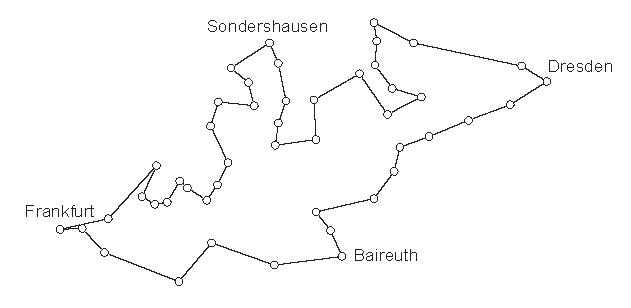
\includegraphics[width=0.9\linewidth]{Immagini/TsP_path.pdf}
    \caption{The Commis-V oyageur tour.}
    \label{fig:TSP_path}
\end{figure}

\noindent The first mathematical papers on the Traveling Salesman Problem (TSP) date back to 1940. Initially, researchers focused on finding a lower bound for the optimal tour. This interest was sparked by a practical problem encountered during an expedition in Bengal, where the transportation of men and materials between locations was a major expense.\\

\newpage

\noindent Mathematicians subsequently generalized the problem, first considering a finite number of random points within a unit-sided square, and later expanding to a general area. During this period, Ghosh observed that the problem proved to be extremely complex, except for very small instances, which, although solvable, held little practical significance. \\

\noindent The term "Traveling Salesman Problem" (TSP) was first mentioned in a 1949 report by Julia Robinson, but it is likely that the name was already in use at Princeton in the 1930s or 1940s. In the 1940s, mathematicians at RAND Corporation, including Merrill Flood, began studying the problem in earnest. In 1954, a team of researchers at RAND, including Dantzig, Fulkerson, and Johnson, made a significant breakthrough by solving a 49-city problem in the USA using the simplex method.

Since then, improvements in solving the TSP have come mainly from developing better methods for applying the cutting plane method to linear programming problems. While there have been no major theoretical breakthroughs, researchers have made progress in understanding the TSP polytope and its properties, as well as developing heuristic algorithms to find near-optimal solutions. A notable theoretical result is the proof of the NP-hardness of the decision version of the TSP in 1972.

In the 1990s, Applegate, Bixby, Chvátal, and Cook developed the program Concorde that has been used in many recent record solutions. Gerhard Reinelt published the TSPLIB in 1991 \cite{TSPLIB95}, a collection of benchmark instances of varying difficulty, which has been used by many research groups for comparing results. In 2006, a team of researchers computed an optimal tour for an 85,900-city instance, currently the largest solved instance. For many other large instances, solutions can be found that are within 2-3\% of an optimal tour \cite{wiki:TSP}.

Today, the research on the TSP is very active and its results have been successfully applied to other Operations Research problems. On one side, there is the search for better heuristics, both for speed and for optimality, using for example simulated annealing, genetic algorithms, tabu-search, neural networks or ant-colonies. On the other side, researchers have developed better and better software to solve the TSP to optimality, mainly through variants of the cutting plane method \cite{fortini2007lp}.


\section{Problem formulation}
The Traveling Salesman Problem (TSP) consists in finding a Hamiltonian circuit of minimum cost on a given directed graph \( G = (V, E) \). In some cases, the problem can be analogously defined on a undirected graph; this happens when the cost associated with an arc does not depend on its orientation \cite{fischetti2019}. In the context of directed graphs, the goal is to find a path that traverses each arc exactly once while minimizing the total cost. Similarly, in undirected graphs, the problem is equivalent when the cost of traversing an edge is symmetric and independent of its direction. \\

\noindent In this document, we primarily address the Symmetric Traveling Salesman Problem (STSP), a fundamental challenge in combinatorial optimization. In STSP, we deal with an undirected weighted complete graph \( G = (V, E) \), where \( V = \{v_1, \ldots, v_n\} \) represents a set of \( n \) nodes, and \( E \) comprises the set of \( (n-1) \) edges. Each edge \( e = \{i, j\} \in E \) is associated with a non-negative real number, represented by the function \( c: E \rightarrow \mathbb{R}^+ \), denoting arbitrary distances or weights between nodes. \\

\noindent As mentioned before, the fundamental goal of the Traveling Salesman Problem (TSP) is to identify the most efficient sequence of edges or nodes that form a tour with the minimum total cost, also known as an optimal tour. To address this task, we need to formulate the problem as an integer linear program. Two notable formulations are the Miller--Tucker--Zemlin (MTZ) formulation and the Dantzig--Fulkerson--Johnson (DFJ) formulation. While the DFJ formulation is stronger, the MTZ formulation remains useful in specific contexts \cite{wiki:TSP}.

\newpage

\subsection{Dantzig–Fulkerson–Johnson (DFJ)}
\label{chap:DFJ}
In this paper, we consider the Dantzig–Fulkerson–Johnson formulation. It is constructed as follows: each city is identified by a unique label from \(1, \ldots, n\), and the cost (or distance) of traveling from city \(i\) to city \(j\) is represented by the positive value \(c_{ij} > 0\). The central variables in this model are \(\{x_{ij}\}_{i,j}\), where \(x_{ij}\) represents the decision variable associated with traveling from city \(i\) to city \(j\). They are constructed as follows:

\begin{align}
    x_{ij} = 
    \begin{cases}
        1 & \text{the path goes from city $i$ to city $j$} \\
        0 & \text{otherwise}
    \end{cases}
\end{align}

The presence of $0/1$ variables in this formulation transforms them into integer programs, while all other constraints remain linear. Specifically, the objective of the program is to minimize the total tour length, which is represented by:

\begin{align}
    \quad \sum_{i=1}^{n} \sum_{\substack{j \neq i \\ j=1}}^{n} c_{ij} x_{ij}.
\end{align}

Without additional constraints, the variables $\{x_{ij}\}_{i,j}$ would essentially span all possible subsets of edges, which is far from the edges that form a tour. This would allow for a trivial minimum solution where all $x_{ij} = 0$. To avoid this, the formulation include the constraints that each vertex has exactly one incoming edge and one outgoing edge, which can be represented by $2n$ linear equations.
The optimization problem is defined as follows:

\begin{align}
    \text{min} \quad & \sum_{e \in E} c_e x_e \label{eq:eq1}\\ 
    \quad & \sum_{e \in \delta(v)} x_{e} = 2 \quad \forall v \in V \label{eq:eq2}\\
    & \sum_{e \in \delta(Q)} x_{e} \leq |Q| - 1 \quad \forall \ Q \subset V:|Q| \geq 2 \label{eq:eq3}\\
    & 0 \leq x_e \leq 1 \text{ integer} \quad \forall e \in E \label{eq:eq4}
\end{align}

\noindent Constraints \ref{eq:eq2} ensure that each node in the graph is visited by exactly two edges of the cycle. 

\newpage

\noindent However, these constraints alone are not sufficient to guarantee a valid Hamiltonian Cycle, as the solution may consist of multiple isolated cycles. The final constraint in the DFJ formulation \ref{eq:eq3}, also known as a Subtour Elimination Constraint (SEC), ensures that any solution found using this model consists of a single connected component. Specifically, this constraint prevents any proper subset \( Q \) from forming a sub-tour, ensuring that the solution is a single tour rather than a collection of smaller tours. Due to the exponential number of possible constraints, the problem can be very difficult to solve so this is typically solved using row generation in practice \cite{wiki:TSP}.
    \chapter{Heuristics}
As the number of nodes in a problem increases, the execution of exact algorithms becomes increasingly computationally demanding. Consequently, heuristic algorithms are employed, which do not guarantee an optimal solution but provide a satisfactory one with reasonable computational cost. We will introduce two families of heuristics:

\begin{itemize}
    \item \textbf{Constructive heuristics}: Generate an approximate solution from scratch.
    \item \textbf{Refinement heuristics}: Improve an existing solution.
\end{itemize}

Constructive heuristics build a solution in a feasible amount of time, typically achieving within 15-20\% of optimality. These heuristics are often used as a starting point for other heuristics, as the quality of the final solution heavily depends on the initial instance.

\section{Nearest Neighbors}
This constructive heuristic algorithm is a greedy 2-approximation algorithm, meaning that the solution is at most 100\% away from the optimum. It generates a solution for the TSP instance in \(O(n^2)\) time, starting from one node and selecting the next node in the tour that is closest to the current node at each iteration \cite{article} \cite{inproceedings}. The step of this algorithm are the following:

\begin{enumerate}
    \item Select a random node.
    \item Find the nearest unvisited node and go there.
    \item If there are any unvisited nodes left, repeat step 2.
    \item Return to the first node.
\end{enumerate}

The pseudocode for computing a single starting solution from an arbitrary node is shown in Algorithm~\ref{alg:NN_algo}.\\

\begin{algorithm}
    \caption{Nearest Neighbour}
    \label{alg:NN_algo}
    \begin{spacing}{1.2} % Adjust this value to change line spacing
        \KwIn{Starting node}
        \KwOut{A valid tour}
        \BlankLine
        path $\leftarrow \{\}$\;
        current\_node $\leftarrow starting\_node$\;
        visited $\leftarrow \{starting\_node\}$\;
        solution $\leftarrow 0$\;
        \While(\tcc*[f]{While there are unvisited nodes}){$|visited| \neq N$}
        {
            closest\_node $\leftarrow $ nearest node \KwTo $current\_node \notin$ visited\;
            solution $\leftarrow solution$ $+$ $dist(closest\_node$, $current\_node)$\;
            current\_node $\leftarrow closest\_node$\;
            \textbf{add} $current\_node$ \KwTo $visited$\;
            \textbf{add} ($current\_node$, $closest\_node$) edge \KwTo $path$\;
        }
        \textbf{add} ($current\_node$, $starting\_node$) edge \KwTo $path$\;
        $solution \leftarrow solution $ $+$ $dist(starting\_node$, $current\_node$)\;
        \BlankLine
    \end{spacing}
\end{algorithm}

Despite its simplicity and speed of implementation, this algorithm often find suboptimal solutions. However, these limitations can be mitigated using improvement techniques such as the 2-opt algorithm, which further enhances the quality of the obtained solution.

\newpage

\subsection{Nearest Neighbors from each node}
An enhanced version of the algorithm can be developed by initiating the process from each possible node. This adjustment brings the complexity to \(O(n^3)\), which is still significantly more efficient than the exponential complexity of exact algorithms. This modification mitigates the algorithm's sensitivity to initial conditions, thereby increasing its robustness. The pseudocode for this enhanced approach is as follows Algorithm~\ref{alg:NN2_algo}:

\begin{algorithm}
    \caption{Nearest Neighbour From Each Node}
    \label{alg:NN2_algo}
    \begin{spacing}{1.2} % Adjust this value to change line spacing
        \KwIn{TSP istance}
        \KwOut{A valid tour}
        \BlankLine
        path $\leftarrow \{\}$\;
        \ForEach{node n}
        {
            current\_path $\leftarrow NearestNeighbors(starting\_node\=n)$\;
            \BlankLine
            \If{current\_path \textbf{better than} path}{
                path $\leftarrow current\_path$\;
            }
        }
        \BlankLine
    \end{spacing}
\end{algorithm}

\section{Refinement Heuristics with 2-Opt}
Once a tour has been generated by a construction heuristic, it can be improved using methods like the 2-opt local search. This kind of heuristic starts from a given solution and improves it by making small changes. Their performances are strongly dependent on the construction heuristic used. Other metaeuristics methods to enhance the solution include tabu search \ref{chap:tabusec} and simulated annealing, both of which utilize the 2-opt move to find neighboring solutions.

This heuristic proposed in 1958 by G. A. Croes \cite{2opt}, first use some construction algorithm and then iteratively improves this tour by resolving crossing edges (\ref{fig:crossing_edge}). This is done by selecting an edge \((v_1, v_2)\) and searching for another edge \((v_3, v_4)\),(the edge \(v_{i}\) belong to the tour) completing a move only if:

\[ \text{dist}(v_1, v_2) + \text{dist}(v_3, v_4) > \text{dist}(v_2, v_3) + \text{dist}(v_1, v_4) \]

\begin{figure}[H]
    \centering
    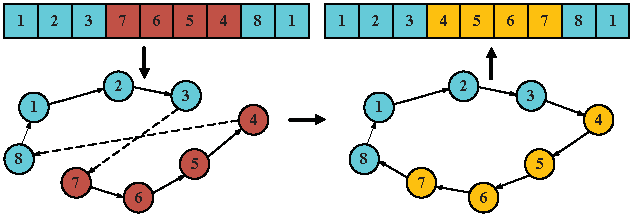
\includegraphics[width=0.9\linewidth]{Immagini/Crossing edges.pdf}
    \caption{Illustration of the process for removing an intersection in a path.}
    \label{fig:crossing_edge}
\end{figure}

This ensures a valid tour, as shown in Figure~\ref{fig:2opt_before_after}. The process continues until no more 2-opt improvements can be found, resulting in a 2-optimal tour. \\

\begin{figure}[H]
    \centering
    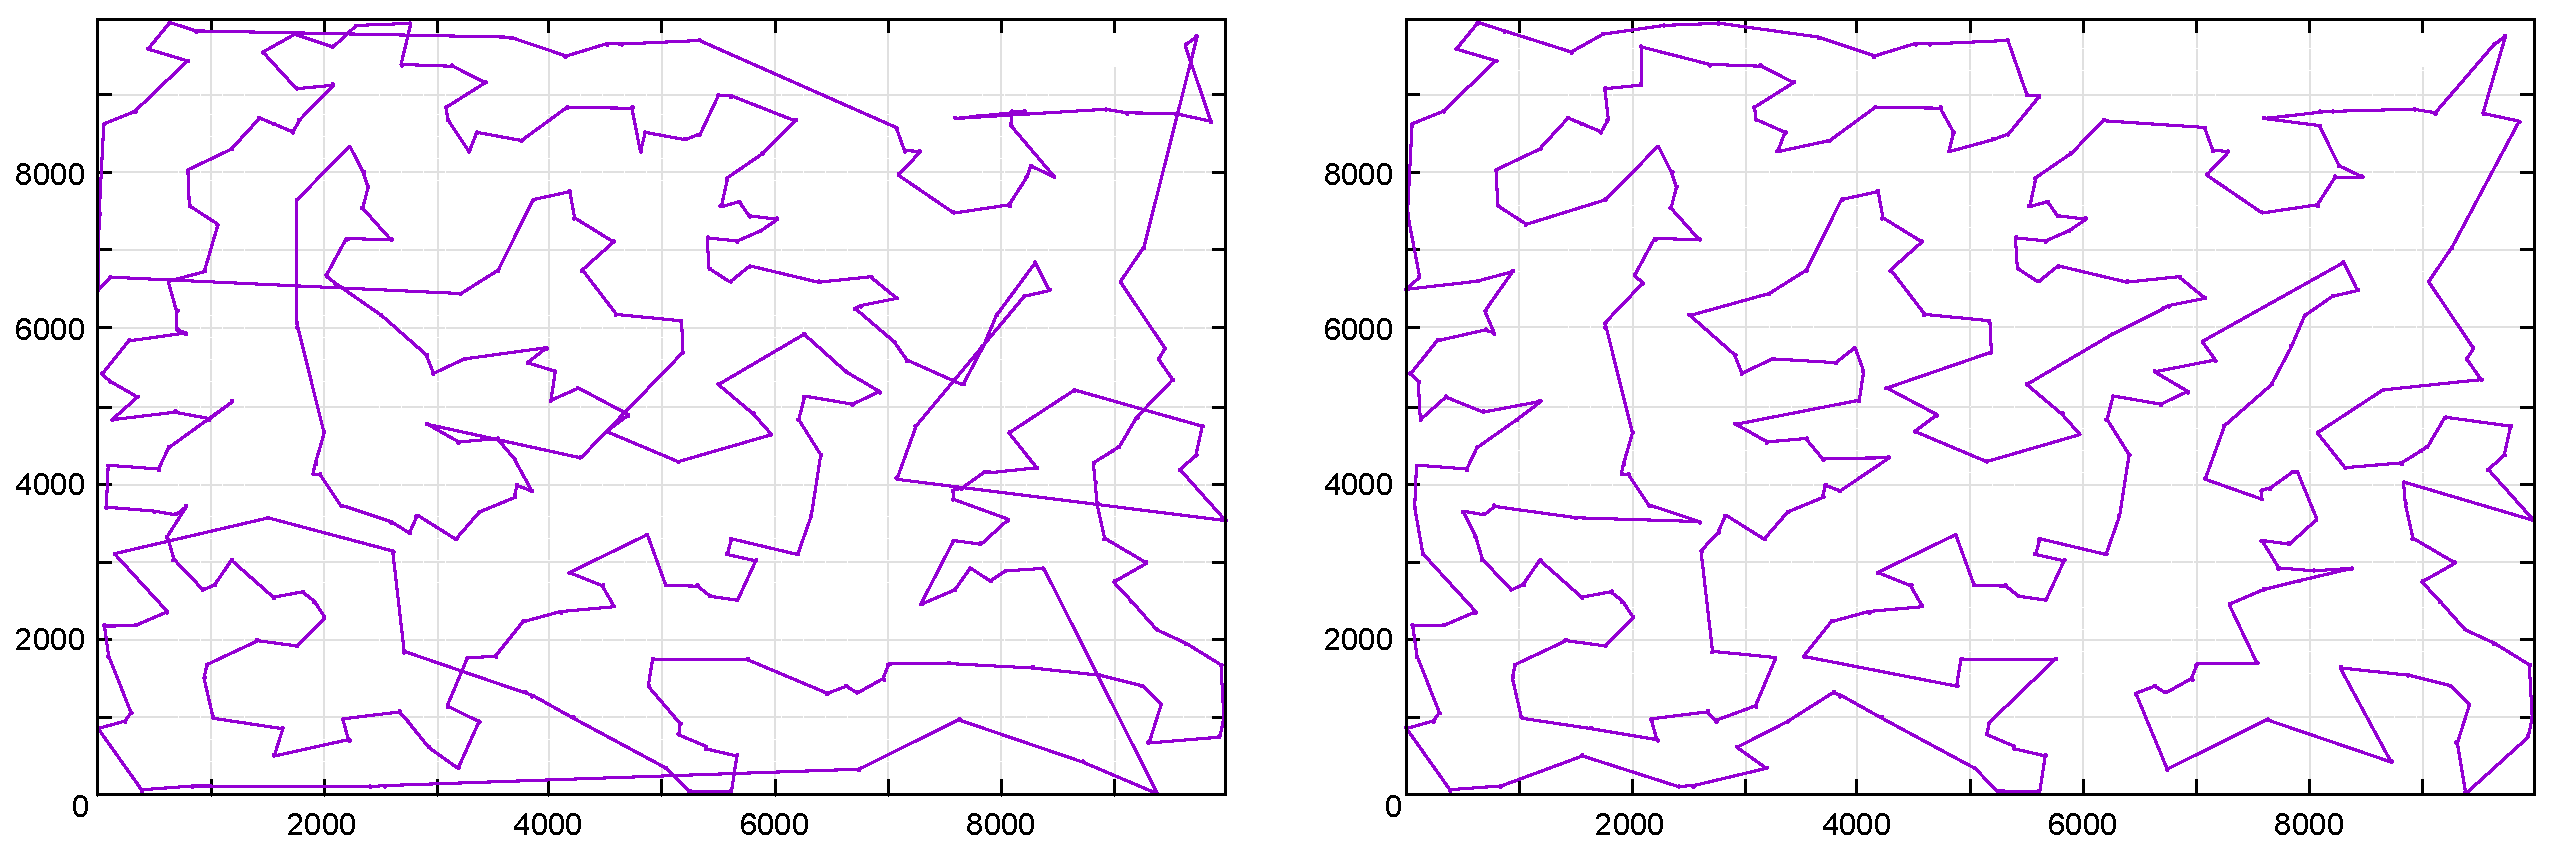
\includegraphics[width=\linewidth]{Immagini/NN+2opt.pdf}
    \caption{2-opt before (left) and after (right)}
    \label{fig:2opt_before_after}
\end{figure}

% \begin{figure}[htbp]
%     \centering
%     \begin{subfigure}[b]{0.48\textwidth}
%         \centering
%         \includesvg[width=\textwidth]{Immagini/svg/NN.svg}
%         \caption{Before}
%         \label{fig:2opt_before}
%     \end{subfigure}
%     \hfill
%     \begin{subfigure}[b]{0.48\textwidth}
%         \centering
%         \includesvg[width=\textwidth]{Immagini/svg/NN+2opt.svg}
%         \caption{After}
%         \label{fig:2opt_after}
%     \end{subfigure}
%     \caption{2-opt before and after}
%     \label{fig:2opt_before_after}
% \end{figure}

\newpage

\noindent The 2-OPT algorithm is shown in Algorithm~\ref{alg:2OPT_algo}.

\begin{algorithm}[H]
    \caption{2-Opt}
    \label{alg:2OPT_algo}
    \begin{spacing}{1.3}
        \KwIn{A valid tour}
        \KwOut{An optimized valid tour}
        \BlankLine
        counter \leftarrow $0$\;

        \While{counter < \#nodes \textbf{and} time < time\_limit}
        {
            counter \leftarrow $counter + 1$\;

            A \leftarrow $tour[0]$\;
            A1 \leftarrow $tour[1]$\;
            \BlankLine
            \For{B \textbf{from} $tour[2]$ \textbf{to} $|tour| -2$}
            {
                B1 \leftarrow $B + 1$\;

                $\Delta(A,B) \leftarrow (c_{A,B} + c_{A1,B1}) - (c_{A,A1} + c_{B,B1})$\;
                \BlankLine
                \If{$\Delta(A,B) < 0$}
                {
                    \tcc{Reverse subvector from A1 to B}
                    \textbf{reverse subvector} $tour[A1 : B]$

                    tour.cost \leftarrow $tour.cost$ + $\Delta(A,B)$

                    \If{current solution better than official solution}
                    {
                        update official solution\;
                    }
                }
            }
            \BlankLine
            move A to the end of the array\;
        }
        \BlankLine
    \end{spacing}
\end{algorithm}

\newpage

\section{Comparison between Heuristics}
As shown in Figure \ref{fig:2opt_before_after}, the result can vary significantly in terms of route and therefore cost, as all possible intersections are eliminated thanks to the 2-opt method, as previously mentioned. However, this may in turn lead to an increase in processing time to remove the intersections and find a better route, in particular with large input files.

Figure \ref{fig:NN_2opt} illustrates the performance profile with the cost comparison between the Nearest Neighbor and the Nearest Neighbor with 2-opt. We can see that the 2-opt gives better result, with an error less the 10\% in every class, while the Nearest Neighbor alone reaches a 20\% in most cases.

\begin{figure}[H]
    \centering
    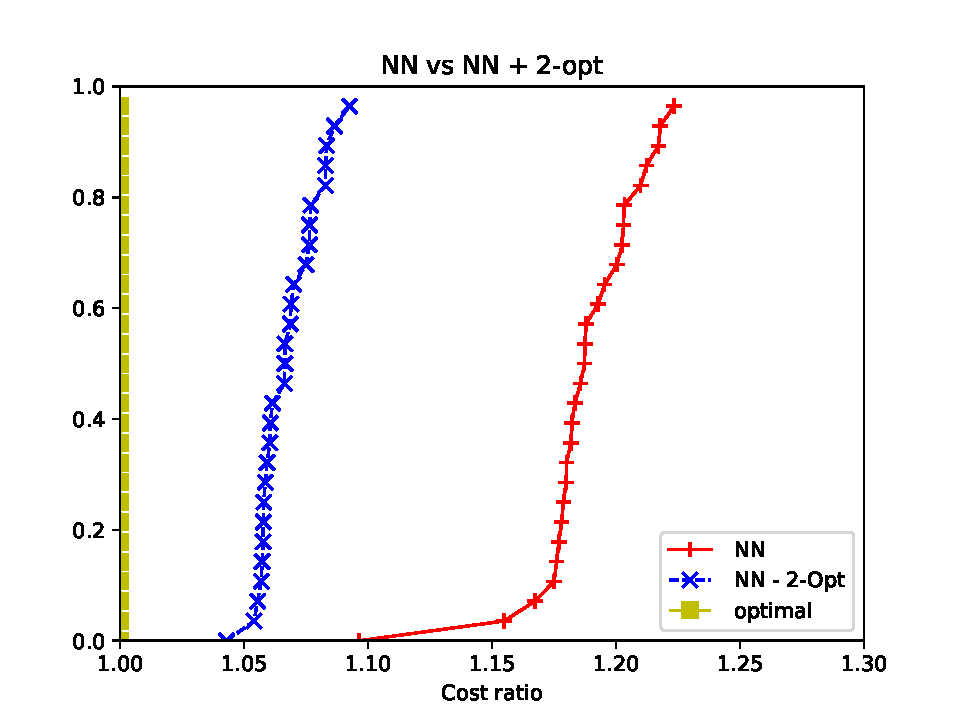
\includegraphics[width=0.7\linewidth]{Immagini/NN vs 2Opt.pdf}
    \caption{Performance Profile of Nearest Neighbor and Nearest Neighbor with 2-opt.}
    \label{fig:NN_2opt}
\end{figure}

    \chapter{Metaheuristics}
Metaheuristics are high-level, problem-independent algorithmic that perturb the solution by moving it away from the current local optimum and attempting to get as close as possible to the global optimum. These algorithms can address various types of optimization problems with minimal adaptation. Even with a basic adaptation to a specific problem, they can often yield good solutions for certain instances. Specifically for the TSP, metaheuristics can typically find better solutions than any 2-opt variation within a reasonable time limit. These techniques essentially allow for the exploration of the solution space, avoiding stagnation in local minima or maxima with objective function values that are far from the global optimum.

In the following sections, we will present two different metaheuristic algorithms:
\begin{itemize}
    \item \textbf{Tabu Search}: When a local minimum is reached adds certain edges to a tabu list, making them forbidden for an improving move. And force the exploration of new situations.
    \item \textbf{Variable Neighborhood Search (VNS)}: Randomly alters \( k \) different edges from the current solution and improves it using 2-opt.
    %\item \textbf{Genetic Algorithm}: Simulates Darwin's theory of evolution, aiming to generate the %fittest population, which may contain a good solution.
\end{itemize}

\section{Tabu Search}
\label{chap:tabusec}
Designed by Fred W. Glover \cite{tabusearch}, the Tabu Search algorithm allows for modifying a given local optimum solution, even at the cost of worsening it, with the goal of exploring the solution space more thoroughly. At each iteration of the algorithm, the solution is modified with a new tour belonging to its 2-opt neighborhood.

To prevent these modifications from leading to the exploration of already visited local minima, a list of ''forbidden moves'' is created, called \(Tabu\) \(List\), which is a FIFO (First In First Out) queue with a specific size. The size of the tabu list is referred to as \(tenure\). This way, a move won’t remain illegal forever but just for a certain number of iterations. 

The performance of this algorithm can depend on the tenure of the list. If it is too small, the algorithm gets stuck in the local minimum because there is a sequence of moves that brings the solution back to the local minimum. Conversely, if the tenure is too large, the search is not effective because the neighborhood is too small.To overcome this, there are some options to dynamically adjust the tenure during execution.\\

There are many different policies to change the Tabu tenure dynamically. The policies considered in this case were:
\begin{itemize}
    \item \textbf{Step policy}: Changes the Tabu List size every \(K\) iterations to a minimum or a maximum.
    \item \textbf{Linear policy}: The Tabu List size grows by 1 unit for each iteration until reaching the maximum size, then decreases by 1 unit for each iteration until reaching the minimum size, and so on.
    \item \textbf{Random policy}: Changes the Tabu List size every \(K\) iterations to a random size chosen within a range.
    \item \textbf{Reactive policy}: The maximum tenure is equal to \(1/K\) (with \(K\) arbitrary) of the number of nodes of the instance to be solved, while the minimum is equal to half of this value.
    \item \textbf{Static policy}: The value of the tenure does not change during the execution.
\end{itemize}

The variant implemented in the code is the \(Static\) \(Policy\), that is the simplest one. A dynamic policy may create better results in theory, but it also requires more computation time. In average, with our input sizes, it should make almost no difference, so we went for the simplest solution.\\

When, during the execution, the method encounters an edge that is tabu, it skips that edge. This ensures that other solutions are explored rather than reverting to the previous ones. When the best non-tabu couple of edges is found, the algorithm does a 2-opt step. It may happen that the best non-tabu swap is a worsening 2-opt move, it would mean that the algorithm reached a local minimum and it is trying to escape from it. 
When the tabu list is full and the method needs to add a new node, the oldest one is removed to make space.
The termination criterion for the algorithm can be defined by either the expiration of the available time or the achievement of a maximum number of iterations. In our code, we used the time-based criterion. The solution provided by the algorithm is the best one identified up to the point of termination.

\newpage

\noindent The Tabu Search pseudocode is shown in Algorithm~\ref{alg:tabu_algo}.

\begin{algorithm}
    \caption{Tabu Search}
    \label{alg:tabu_algo}
     \begin{spacing}{1.2} % Adjust this value to change line spacing
        \KwIn{TSP Istance with a feasible solution}
        \KwOut{A valid tour}
        \BlankLine
        result $\leftarrow$ best solution found so far\;
        cost $\leftarrow$ cost of result\;
        tenure $\leftarrow \max(\text{inst.nnodes} / 10, 10)$\;
        \BlankLine
        \While{time elapsed $<$ time\_limit}
        {
            \ForEach{node pair (A, B)}
            {
                \textbf{if} \textit{A or B in TabuList} \textbf{then Skip}\;

                \BlankLine
                compute \KwSty{swap} costs\;
                \If{fist iteration \textbf{or} new cost $<$ bestCost}
                {
                    bestSol $\leftarrow$ updated solution\;
                    bestCost $\leftarrow$ new cost\;
                    swappedNode $\leftarrow$ node A\;
                }
            }
            \BlankLine
            \If{bestCost $\geq$ cost}
            {
                \KwSty{add} swappedNode \KwTo tabu list\;
            }
            \BlankLine
            result $\leftarrow$ bestSol\;
            cost $\leftarrow$ bestCost\;
        }
    \end{spacing}
\end{algorithm}

\section{Variable Neighborhood Search (VNS)}
The Variable Neighborhood Search (VNS) algorithm, introduced by N. Mladenović and P. Hansen \cite{MLADENOVIC19971097}, aims to enhance a given local optimum by starting with an arbitrary solution and exploring neighborhoods of different sizes, as illustrated in Figure~\ref{fig:vns}. 
The idea of the VNS algorithm is that Tabu Search waste too much time to escape from a local minimum. 

\newpage

\noindent That time should instead be used for optimization. That is why it uses a quick way of escaping: the kick. This method is also a less controllable way that does not assure good results since it may fall back to the same local minimum.
VNS is founded on three key principles:

\begin{itemize}
    \item A local minimum in one neighborhood structure may not be the same in another.
    \item A global minimum is a local minimum in all neighborhood structures.
    \item Often, a local minimum in one neighborhood structure is near a local minimum in another.
\end{itemize}

\begin{figure}[H]
    \centering
    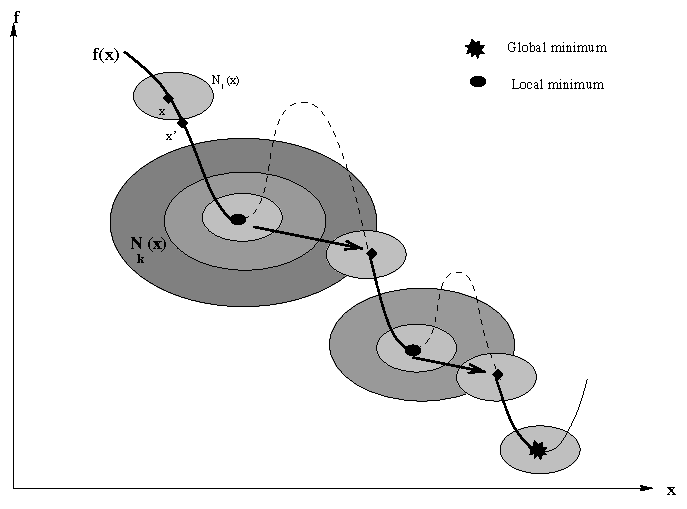
\includegraphics[width=0.65\linewidth]{Immagini/vns.pdf}
    \caption{An illustration of the Variable Neighborhood Search (VNS) process \cite{Hansenvns}.}
    \label{fig:vns}
\end{figure}

If a superior solution is not discovered in the neighborhoods of size \( K \), the algorithm randomly selects and replaces certain branches with other edges \cite{Hansen2019}. This introduces a temporary increase in cost, with the expectation that a new neighborhood will lead to a solution that diverges from the initial local optimum.

VNS repeatedly refines the current solution until a local minimum is achieved (intensification phase), using the 2-opt method. Subsequently, the algorithm picks a random solution within the neighborhood (diversification phase) as shown in the Figure~\ref{fig:vns_kick}. If this new solution is better than the best one found so far, it becomes the new best solution. In the next iteration, the algorithm starts with the smallest neighborhood; if no improvement is found, it moves to a larger neighborhood.

\begin{figure}[H]
    \centering
    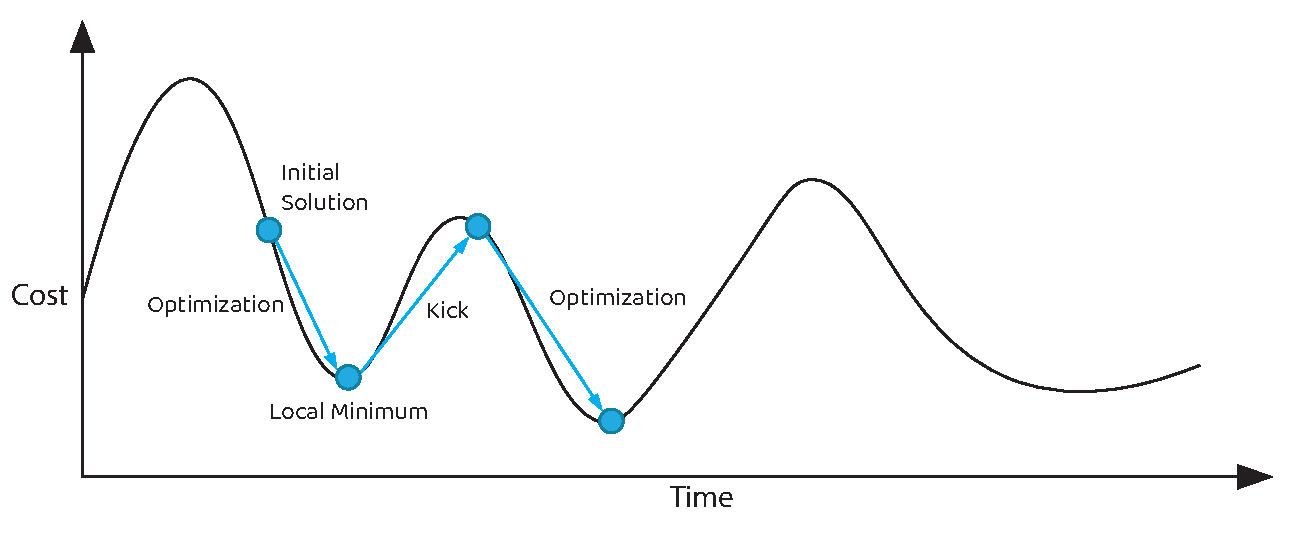
\includegraphics[width=0.85\linewidth]{Immagini/vns-kick.pdf}
    \caption{An illustration of the Variable Neighborhood Search (VNS) process.}
    \label{fig:vns_kick}
\end{figure}

The algorithm \ref{alg:vns_algo} concludes when a user-defined time limit is reached or after a set number of iterations, returning the best solution found. This method retains much of the initial solution, preventing the loss of previously gathered information.

\begin{algorithm}[H]
    \caption{Variable Neighborhood Search}
    \label{alg:vns_algo}
    \begin{spacing}{1.2} % Adjust this value to change line spacing
        \KwIn{TSP instance}
        \KwOut{A valid tour}
        \BlankLine
        Initialize result vector with best solution found so far\;
        \While{time < time\_limit}
        {
            performTwoOptOptimization()\;
            \For{$i \leftarrow 1$ \KwTo random number between 2 and 10}
            {
                applyKick()\;
            }
        }
        \BlankLine
    \end{spacing}
\end{algorithm}

The implementation presented here considers only the 3-opt neighborhood. This means that during the kick operation \ref{alg:kick_func}, three edges are randomly removed and reconnected in a predefined manner.

\begin{algorithm}[H]
    \caption{Kick Function \textit{applyKick()}}
    \label{alg:kick_func}
    \begin{spacing}{1.2} % Adjust this value to change line spacing
        \KwIn{Solution vector, cost}
        \KwOut{Updated solution vector and cost}
        Randomly select indices $i$, $j$, $k$\;
        Update the solution vector by swapping sub-sections between $i$ and $j$ and between $j$ and $k$\;
        Adjust the cost based on the new configuration\;
        \BlankLine
    \end{spacing}
\end{algorithm}

\section{Comparison between Metaheuristics}
We have seen two important metaheuristic algorithms applied to the TSP. Here we compare the two algorithms in terms of costs of the solution found.

Figure \ref{fig:tabu_vns} illustrates the cost comparison between our implementation of the Tabu Search algorithm and the Variable Neighborhood Search (VNS) algorithm. Both were given a time limit of 60 seconds.

As we can see they gave mostly the same results. The ability of VNS to outperform Tabu Search in some cases suggests that it can offer advantages in certain situations, though not consistently. Similarly, the inferior performance of VNS in other cases indicates that Tabu Search maintains a competitive robustness. Overall, this analysis confirms the qualitative equivalence of the two implementations in our application context.

\begin{figure}[H]
    \centering
    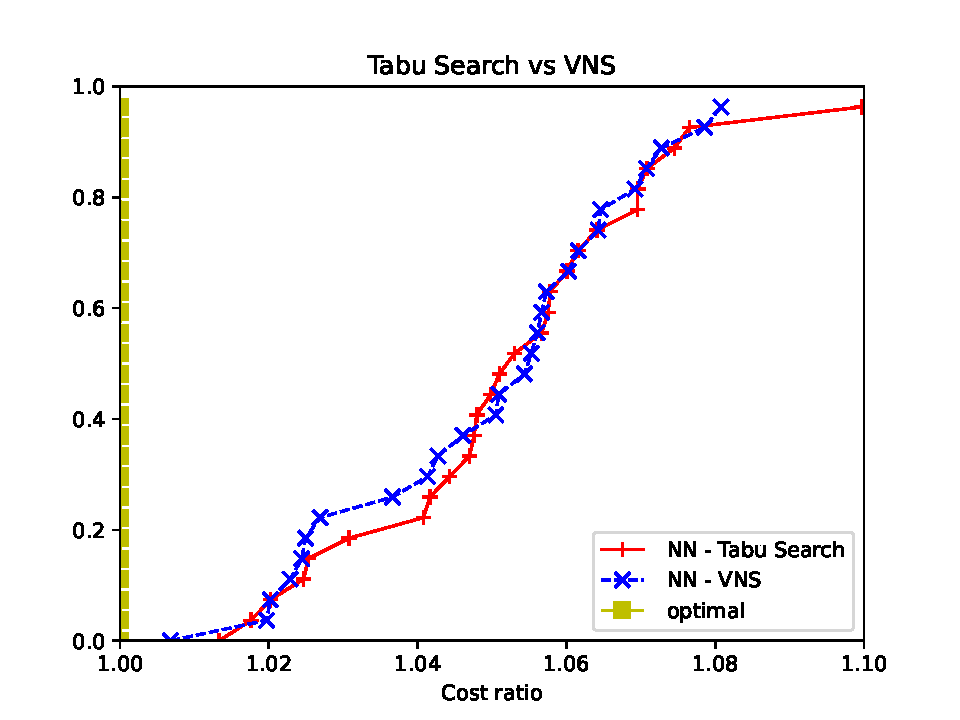
\includegraphics[width=0.7\linewidth]{Immagini/Tabu vs VNS.pdf}
    \caption{Performance Profile of Tabu Search and VNS.}
    \label{fig:tabu_vns}
\end{figure}

    
\chapter{Exact Models}
The previous sections illustrated some heuristic methods. The main property of those methods is their speed, but they provide approximate solutions. In contrast, to obtain the best possible solution, we must use exact methods that optimize a mathematical model of the problem and find the optimal solution.

This section introduces methods that solve a MIP problem to optimality using the basic CPLEX \cite{Cplex:TSP} MIP solver. The MIP problem model used is described in the introduction section \ref{chap:DFJ}.

The main challenge was adding the sub-tour elimination constraints (SEC) \ref{eq:eq3}. The initial approach was to define and build a model without these constraints and directly use the CPLEX solver on it. Obviously, this approach yields an incorrect solution composed of various separated components instead of a unique path that visits all points.

To address this problem, the first method that we propose is Benders' Loop, which iteratively adds the SEC and solves the problem until the optimal solution without subtours is found. The second method uses a CPLEX callback function that is called every time a new solution is found. This allows us to reject solutions with subtours by adding the corresponding SECs or to accept the solution if it has only one component.
We will also cover some other methods that can speed up the process, such as Posting heuristic solutions, MIP start and User-cut callbacks.

\section{Benders' Loop method}
The Dantzig-Fulkerson-Johnson (DFJ) \ref{chap:DFJ} model incorporates subtour elimination constraints to the problem, but the number of such constraints is exponential.

The first method we introduce to address this issue is known as "Benders' Loop". This method is based on the idea that the majority of potential subtours consist of very unfavorable edge combinations, which correspond to parts of the solution space that the MIP solver would quickly discard while minimizing the solution cost. Therefore, the method focuses only on the subtours selected by the solver, prohibiting their selection.

Benders' implementation iteratively solves the DFJ model. It begins with the degree constraints and solves the problem using CPLEX's MIP solver. Upon finding a solution, it checks for the presence of subtours. If subtours are detected, the method adds subtour elimination constraints (SECs) for each subtour and resolves the modified model until a solution is found or the time limit is reached. Specifically, if the solution contains \( m \) subtours and \( S_k \) is a subtour, the Loop method adds the following constraints:

\[
\sum_{e \in E(S_k)} x_e \leq |S_k| - 1 \quad \text{for} \; k = 1, \ldots, m
\]

The pseudo-code of Benders’ loop method is shown in Algorithm~\ref{alg:Bender}.

\begin{algorithm}[H]
    \caption{Benders implementation of the DFJ model}
    \label{alg:Bender}
    \begin{spacing}{1.2} % Adjust this value to change line spacing
        \KwIn{TSP instance}
        \KwOut{A valid tour (CPLEX solution)}
        \BlankLine
        model \leftarrow $naive\_model$\;
        solution \leftarrow $solve$ model\;

        \While{solution \textbf{has} $subtours$}
        {
            \ForEach{subtour \textbf{in} solution}
            {
                sec\_constraints \leftarrow generate SECs constraints of subtour\;
                \textbf{add} sec\_constraints \textbf{to} model\;
            }
            solution \leftarrow $solve$ model
        }
        \BlankLine
    \end{spacing}
\end{algorithm}

This procedure avoids generating an exponential number of constraints. However, the major drawback is the need to rebuild and reoptimize the model from scratch at each iteration.

\subsection{Patching Heuristic for Benders: Gluing}
The Bender's Loop method, in every iteration, only creates new SECs and then discards all previous work to start again from scratch. Instead, it would be beneficial to save as much progress as possible to make the method more efficient. A possible solution is to attempt to fix the solution provided by CPLEX by gluing together the subtours, resulting in a single comprehensive path.

The output of this technique will not have any guaranteed optimality, but it could still be valuable. In case the method is stopped before completion, we would have a feasible solution. Additionally, it can provide a good upper bound, as we know that the optimal solution will have a cost better than or equal to the glued solution. Moreover, it offers a good starting point for the next iteration, as the glued solution can be provided to CPLEX as a MIP start.

The action of gluing together two subtours is made by choosing the best couple of edges of different components that generate the lowest difference of cost when swapped (as shown in Figure \ref{fig:patch_img}). This operation is repeated until there is only one component.

\begin{figure}
    \centering
    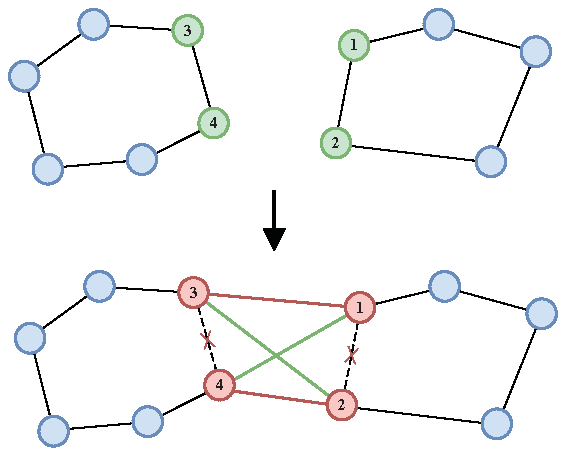
\includegraphics[width=0.8\linewidth]{Immagini/patch.pdf}
    \caption{Gluing of two components.}
    \label{fig:patch_img}
\end{figure}

\newpage

The pseudo-code of the gluing operation is shown in Algorithm~\ref{alg:gluing}. It takes as input the multi-component solution in a particular format:
\begin{itemize}[noitemsep]
    \item \texttt{ncomps}: number of components
    \item \texttt{comp}: array with ids of components for each node
    \item \texttt{succ}: array with successive node of each node
    \item \texttt{cost}: cost of the current solution
\end{itemize}

\begin{algorithm}[H]
    \caption{Gluing}
    \label{alg:gluing}
    \begin{spacing}{1.3} % Adjust this value to change line spacing
        \KwIn{ncomps, comp, succ, cost}
        \KwOut{The glued solution}
        \BlankLine
        \While{\textit{ncomp > 1}}
        {
            edge1, edge2, costDifference \leftarrow \textbf{find} \ \textit{best (with minimum cost difference) 2 edges to} \textbf{swap} \textit{such that they are from different components}\;
            
            \BlankLine
            \textbf{swap} \textit{succ[edge1.first]} \textbf{with} \textit{succ[edge2.first]}\;
            \textbf{update} value of \textit{comp} to values in range \textit{[1, ncomp-1]}\;

            \BlankLine
            cost \leftarrow \textit{cost + costDifference}\;
            ncomp \leftarrow \textit{ncomp - 1}\;
        }
        \BlankLine
    \end{spacing}
\end{algorithm}

\section{Branch and Cut in CPLEX with candidate callback}

An alternative method to incorporate SEC constraints is through the branch-and-cut technique, specifically utilizing CPLEX to address the problem. 

At the root node, CPLEX’s branch-and-cut algorithm performs several preprocessing steps. For each node in the branching tree (Figure \ref{fig:bec_img}), it employs multiple cut separation families, such as Gomory, Clique, and 0-1/2 cuts. Following the calculation of the relaxation, primal heuristics are applied to identify increasingly optimal incumbent solutions. These heuristics take the fractional solution as input, convert it into an integer solution, and if the resulting cost is lower than the current incumbent solution, the incumbent is updated. This integer solution may still contain subtours. 


\begin{figure}[H]
    \centering
    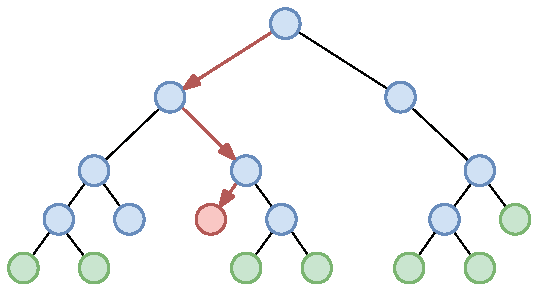
\includegraphics[width=0.9\linewidth]{Immagini/bec.pdf}
    \caption{Branch \& Cut tree visualization.}
    \label{fig:bec_img}
\end{figure}

Between the heuristic application and the incumbent update, it is possible to instruct CPLEX to invoke a custom callback function. Exploiting this CPLEX feature we can inspect the solution and act based on its properties. If it has sub-tours the function adds the SECs and discards the solution, while if it has only one component the function accepts it.

This method let use fully use the potential of CPLEX without needing to restart the optimization multiple times.

The pseudo-code of the candidate callback is shown in Algorithm~\ref{alg:cand_callback}.\\

\begin{algorithm}[H]
    \caption{Candidate callback}
    \label{alg:cand_callback}
    \begin{spacing}{1.2} % Adjust this value to change line spacing
        \KwIn{Candidate solution}
        \BlankLine
        \If{solution \textbf{has} subtours}
        {
            \ForEach{subtour \textbf{in} solution}
            {
                sec\_constraints $\leftarrow$ generate SECs constraints of subtour\;
                \textbf{add} sec\_constraints to model\;
                \textbf{discard} solution\;
            }
        }
        \Else
        {
            \textbf{accept} solution\;
        }
        \BlankLine
    \end{spacing}
\end{algorithm}

\newpage

\subsection{Posting Heuristic solutions}
The incumbent callback allows for the implementation of custom heuristics to help CPLEX quickly identify an improved solution.

Starting with the integer solution provided by CPLEX in this callback, the gluing algorithm from the Bender's loop method can be applied, followed by a 2-opt optimization.

The improved solution can then be \textit{posted} in the CPLEX environment, making it available for evaluation. CPLEX will assess this solution and determine whether to adopt or discard it.

\subsection{MIP start}
In addition to the aforementioned techniques, it is also possible to provide a starting solution to CPLEX, known as a MIP start, which prevents the creation of poor random solutions at the beginning of the Branch-and-Cut (B\&C) method. By doing so, the CPLEX solver can begin its optimization process with a reasonably good feasible solution, working to improve it towards optimality rather than starting from a random solution, which may be much more challenging to optimize.

To generate the MIP start solution, any of the previously discussed heuristic or metaeuristic methods can be employed. In our case, we decided to use a simple nearest neighbor heuristic starting from a random node, combined with a 2-opt optimization: a suitable balance between a fast and robust approach.

\section{SECs for Fractional solutions: user-cut callback}
In this section, we describe an advanced use of CPLEX’s callback functionality. At each node of the branching tree, CPLEX allows the invocation of a user-cut callback, a custom function applied to the relaxed solution of the problem. The relaxed solution does not account for the integer constraints of the variables. This feature facilitates the creation of custom cuts for the relaxed problem using callbacks. However, in the context of the TSP, the solution must be integer. Consequently, the methods used in previous sections to count the number of components or to merge them are not applicable.

To address this, functions from the Concorde library are utilized \cite{conc}. For example, the function \texttt{CCcut\_connect\_components} counts the components in a fractional solution, and \texttt{CCcut\_violated\_cuts} calculates the min-cut of a flow problem. The implemented callback functions, similarly to the candidate callback, use this library to compute the number of components in the relaxed solution returned by CPLEX and, for each component, an SEC is applied as a global constraint.

The distinction from the candidate callback arises when the number of components found is one. In the candidate callback, a solution with one component is considered feasible. However, in the user-cut callback, the min-cut on the graph needs to be calculated. For instance, in TSP, for each cut $(S, V \setminus S)$, the constraint

\begin{equation}
\sum_{(i,j) \in \delta(S)} x_{ij}^* \geq 2 \quad \forall S \subseteq V, S \neq \emptyset
\end{equation}

must be satisfied, where $i \in S$, $j \in V \setminus S$, $x_{ij}^* \geq 0$ is the value of the edge $(i, j)$ in the relaxed solution, and $\delta(S)$ is the cut-set of $S$. The Concorde function \texttt{CCcut\_violated\_cuts} identifies the cuts violating this constraint, and SECs are applied to each cut.

Unfortunately, applying this callback at every node of the branching tree is impractical due to the high time complexity of Concorde’s algorithms. Thus, cuts are applied with a probability of 10\%. An alternative approach could involve applying cuts when the node depth in the branching tree is below a certain threshold (e.g., 5).

It is important to note that User-Cuts callbacks are a subroutine of the candidate callback method. The candidate callback is triggered when an integer solution is found, while user cuts are called for fractional solutions. This helps CPLEX enforce critical constraints before updating the incumbent solution, potentially reducing the branching tree size and overall computation time.

The pseudo-code of the candidate callback is shown in Algorithm~\ref{alg:user_callback}.

\begin{algorithm}[H]
    \caption{user-cut callback}
    \label{alg:user_callback}
    \begin{spacing}{1.2} % Adjust this value to change line spacing
        \KwIn{Fractional solution}
        \BlankLine
        with probability 90\%: \textbf{return}\;
        \textbf{call} \texttt{CCcut\_connect\_components} on solution\;
        \If{number of components \geq 1}
        {
            \ForEach{subtour \textbf{in} solution}
            {
                sec\_constraints $\leftarrow$ generate SECs constraints of subtour\;
                \textbf{add} sec\_constraints to model\;
                \textbf{discard} solution\;
            }
        }
        \Else
        {
            \textbf{call} \texttt{CCcut\_violated\_cuts} on solution\;
        }
        \BlankLine
    \end{spacing}
\end{algorithm}

\section{Comparison between Exact Models}
Figure \ref{fig:benders_comp} illustrates the performance profile with the time comparison between our implementation of the base Benders' loop method and Benders' loop method with gluing.

The two algorithms have similar performances, with some exception where the version with gluing is much slower. This probably happens with the biggest inputs, when the operation of gluing begins to be too heavy. 
In the 80\% of the cases however they took the same time to find the optimal solution, and the gluing feature lets the user have a partial solution even if the algorithm is stopped before finishing.

\begin{figure}[H]
    \centering
    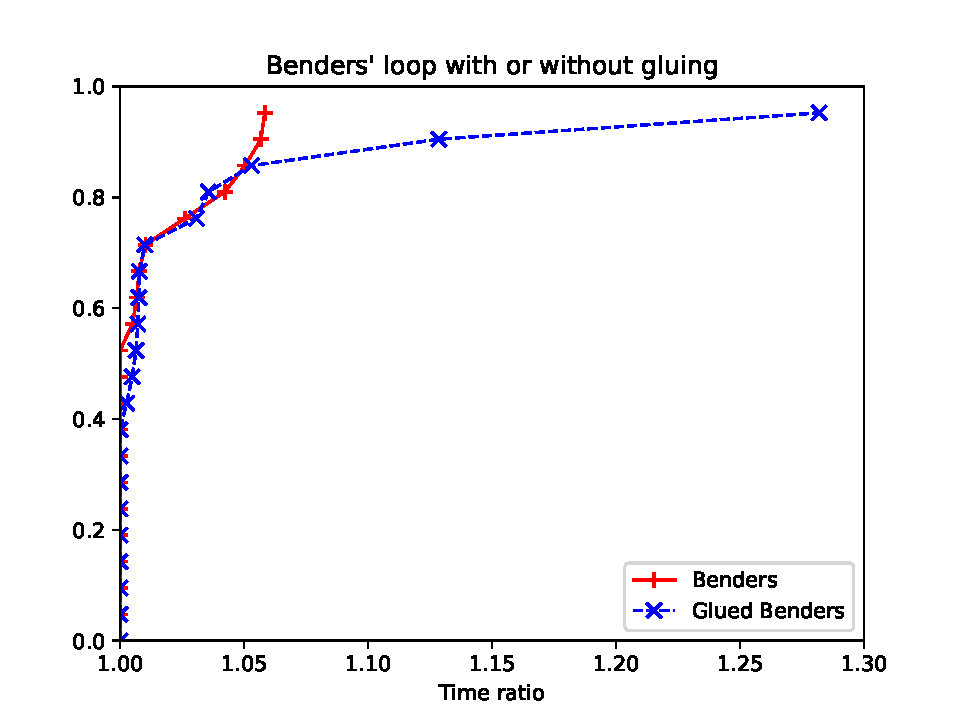
\includegraphics[width=0.7\linewidth]{Immagini/benders.pdf}
    \caption{Performance profile of Benders' loop methods.}
    \label{fig:benders_comp}
\end{figure}

The graph in Figure \ref{fig:benders_comp} compares the performance profiles of the various exact methods described in this section. 

Utilizing all available features, including MIPStart, candidate callback, user-cut callback and posting, yields the best performance, significantly improving the algorithm's efficiency and solution quality. 
Even when using only candidate callbacks and posting without MIPStart and user-cut callbacks, the performance remains highly effective, matching the best results, which indicates that posting is a particularly powerful technique within these methods. 

The B\&C approach with both callbacks is comparable with the Benders' loop method, this indicated that with the modern computational power even a more basic method is capable of performing comparably with the others.

\newpage

Overall, the analysis demonstrates that while Benders' decomposition and B\&C methods are both powerful, the strategic use of enhancements like callbacks, MIP start, and especially posting can significantly influence their performance, making them more efficient and adaptable to real-world scenarios.

\begin{figure}[H]
    \centering
    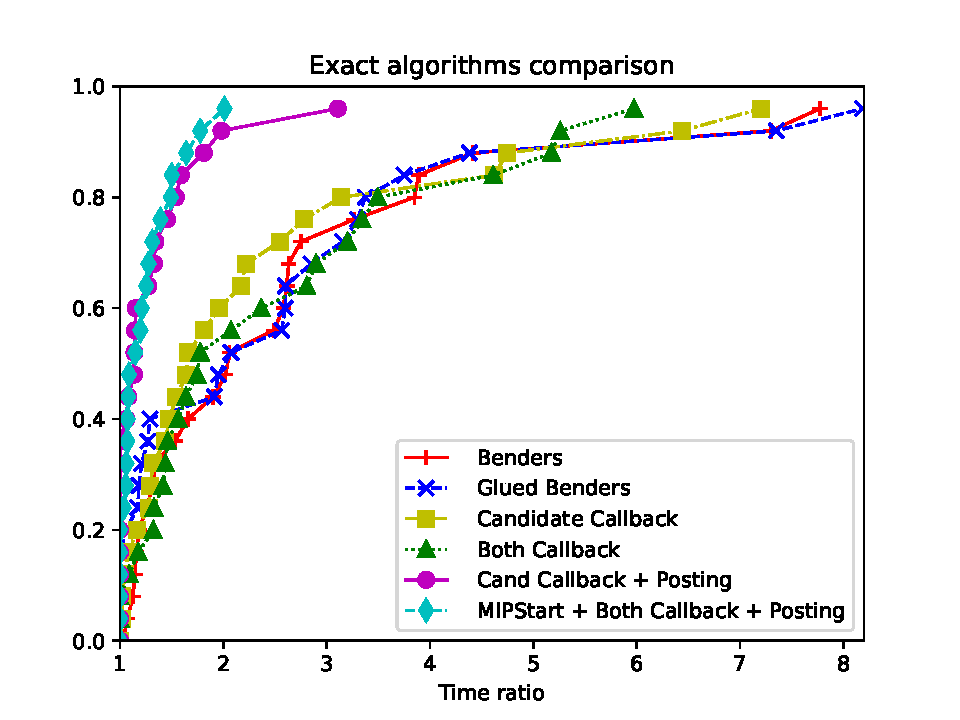
\includegraphics[width=0.7\linewidth]{Immagini/exacts.pdf}
    \caption{Performance profile of all exact methods.}
    \label{fig:exacts_comp}
\end{figure}
    \chapter{Matheuristics}

A heuristic, as defined in \cite{wiki:Heuristic}, is "any approach to problem-solving or self-discovery that employs a practical method, not guaranteed to be optimal, perfect, logical, or rational, but sufficient for reaching an immediate goal. When finding an optimal solution is impossible or impractical, heuristic methods can speed up the process of finding a satisfactory solution." According to this definition, heuristic algorithms aim to find good solutions in a reasonable time by sacrificing optimality.

Matheuristic algorithms combine heuristic methods with mathematical programming, introducing new constraints to the model. In this way the B\&C algorithm is treated as a black box, making the method independent from its implementation and from the problem. The most representative algorithm of this method is Soft Fixing (see Section \ref{chap:local_branching}).

During the solution computation, CPLEX employs various heuristic and matheuristic algorithms. By adjusting certain parameters, it is possible to change the frequency of their application or the time allocated to them.


\section{Hard Fixing}
The Hard Fixing Heuristic is an iterative approach that fixes certain variables (edges) of a reference solution computed by CPLEX and then attempts to solve the resulting simplified problem using a Mixed-Integer Programming (MIP) solver. The heuristic consists of the following steps:

\begin{enumerate}
    \item Start from a solution
    \item Fix used edges to 1 with a certain probability
    \item Run MIP solver as a black box
    \item Compare solutions and keep the best one
    \item Remove fixed edges
    \item Repeat from point 2
\end{enumerate}

These steps are repeated for a fixed number of iterations. Upon finding a solution, the fixed edges are unfixed, and the process is restarted until the time limit is reached. The optimization is accelerated because the fixed edges removes a lot of feasible solutions from the domain (the nodes of a fixed edges have one degree of freedom less than before). However, optimality of the solution is not guaranteed. Importantly, each iteration's solution is at least as good as or better than the previous one.

The heuristic begins by creating the model and calling the MIP start function that generates a solution using Nearest Neighbor and the 2-opt. This initial solution is likely far from optimal, but we use it to choose some random edges and fix them to 1 by adding a costraint \(x_e=1 \) to the model with a certain probability.

The percentage of edges to be fixed varies at each iteration. Generally, a high percentage is used in the initial iterations and is gradually reduced in subsequent ones, allowing CPLEX greater flexibility in computing the solution. The random selection of edges in Phase 2 ensures the algorithm terminates, as the same variables are not always fixed.

In the implemented version, the percentages used are calculated on the fly, based on how much the results improve at each iteration (a low improvement makes the percentage of free edges increase by 10\%, up to 50\%, allowing the solver to have a higher flexibility).

An example of the solution space exploration using this technique is shown in Figure \ref{fig:hrd_fix}. The pseudo-code of the Hard Fixing Heuristic is provided in Algorithm \ref{alg:hard_fixing}.

\begin{figure}[H]
    \centering
    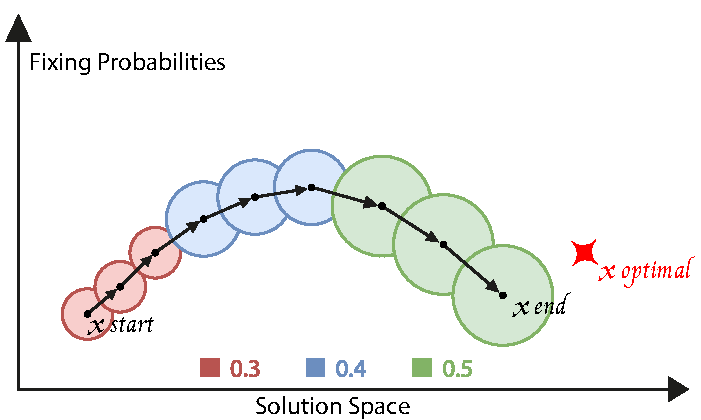
\includegraphics[width=0.8\linewidth]{Immagini/hrd_fix.pdf}
    \caption{Solution space exploration using the Hard Fixing Heuristic.}
    \label{fig:hrd_fix}
\end{figure}

\begin{algorithm}[H]
    \caption{Hard Fixing}
    \label{alg:hard_fixing}
    \begin{spacing}{1.2} % Adjust this value to change line spacing
        \KwIn{TSP Instance}
        \KwOut{A valid tour}
        \BlankLine
        build cplex model\;
        current\_solution $\leftarrow$ addMipStart\;
        freeEdgesProb $\leftarrow$ 0.1\;
        \BlankLine
        \While{current time $<$ inst.time\_limit}
        {
            \ForEach{edge of current\_solution}
            {
                \If{edge $=$ 1}
                {
                    fix edge to 1 with probability 1 - freeEdgesProb\;
                }
            }
            \BlankLine\BlankLine
            \textit{cpx\_solution} $\leftarrow$ \textbf{call} branch\&Bound black box\;
            \BlankLine\BlankLine
            \If{cpx\_solution cost \leq \ current\_solution cost}
            {
                \textit{current\_solution} $\leftarrow$ \textit{cpx\_solution}\;
                addMipStart(\textit{current\_solution})\;
            }
            \BlankLine
            \For{each edge of current\_solution}
            {
                free edge\;
            }
            \BlankLine
            \If{$|$objval - cpx\_objval$| < 0.1 \times$ objval}
            {
                freeEdgesProb $\leftarrow$ min(freeEdgesProb + 0.1, 0.5)\;
            }
        }
    \end{spacing}
\end{algorithm}

\section{Local Branching}
\label{chap:local_branching}

The Local Branching method, also known as Soft Fixing, introduced by M. Fischetti and A. Lodi \cite{Fischetti2003}, adopts an approach similar to Hard Fixing. However, in this technique, the selection of variables to be set to 1 is not done randomly but is determined by CPLEX.

\newpage

\noindent Starting from a feasible integer solution for the TSP, denoted as \(x^H\), which is represented as a binary vector (e.g., [0, 1, 0, ...]) of length \(|E|\), a constraint is applied to the variables with value 1:

\begin{equation}
    \sum_{e \in E\ :\ x_{e}^{H} = 1} x_e \geq n - k
    \label{eq:loc_fix_2}
\end{equation}

where the summation represents the count of variables that are set to 1 in \(x^H\) and will remain unchanged, \(n\) denotes the number of edges selected in \(x^H\) and where \(k = 2, \ldots, 20\) signifies the degrees of freedom for CPLEX in finding the new solution. In each iteration of the algorithm, a new Local Branching constraint is introduced based on the current solution provided by CPLEX, while the constraint from the previous iteration is removed.

Unlike Hard Fixing, where branches are selected randomly, if there is no improvement in cost and thus no change in the solution, the branches chosen by CPLEX with the new constraint would be the same as in the previous iteration. To overcome this, the value of \(k\) starts at 2 and is incremented if the solution does not improve.
Experimental results indicate that this method helps CPLEX converge more rapidly to the optimal solution, and values of \(k\) greater than 20 do not yield better outcomes. Typically, to explore the solution space, it is necessary to enumerate all the elements within it. The addition of a Local Branching constraint simplifies and accelerates this operation.
Given a feasible integer solution \(x^H\) and using the Hamming distance, the \(k\)-opt solutions relative to \(x^H\) are those at a distance \(k\) from it as shown in Figure \ref{fig:soft_fix}.

\begin{figure}[H]
    \centering
    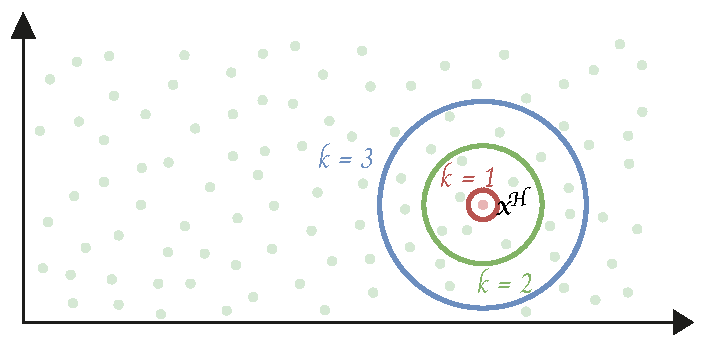
\includegraphics[width=0.8\linewidth]{Immagini/soft_fix.pdf}
    \caption{Solution space and Hamming distance.}
    \label{fig:soft_fix}
\end{figure}

For generic \(k\), approximately \(n^k\) solutions should be generated at a distance \(k\) from \(x^H\). These solutions must be analyzed to find one with a lower cost than \(x^H\).
Local Branching can also be applied to general problems, not just the TSP. Given an approximate (heuristic) solution \(x^H\) for an optimization problem, the mathematical formulation that generates solutions at a distance less than or equal to \(R\) through Local Branching is:

\begin{align}
    min\{c^Tx\ : \ Ax=b,\ x \in \{0,1\}^{|E|}\} \label{eq:loc_fix_2} \\[2em]
    H(x,x^h)\ = \sum_{j \in \{1 ... n\}\ :\ x_{j}^{H}=0} x_j\ + \sum_{j \in E\ :\ x_{j}^{H}=1} (1 - x_j)\ \ \leq R \label{eq:loc_fix_2}
\end{align}

Equation \ref{eq:loc_fix_2} represents the Hamming distance of the new solution \(x\) from \(x^H\). The goal of Soft Fixing is to improve the solution cost by examining the nearest solutions in the space. The algorithm resembles the hard-fix approach, but instead of using the fixing-probability, we modify the neighborhood by adjusting the radius parameter \(k\). The pseudo-code for Soft Fixing is presented in Algorithm \ref{alg:soft_fixing_algo}.\\

\begin{algorithm}[H]
    \caption{Local Branching}
    \label{alg:soft_fixing_algo}
    \begin{spacing}{1.2} % Adjust this value to change line spacing
        \KwIn{TSP Instance}
        \KwOut{An improved solution}
        \BlankLine
        build cplex model\;
        current\_solution $\leftarrow$ addMipstart\;
        $k \leftarrow 20$\;
        \BlankLine
        \While{current time $<$ inst.time\_limit}
        {
            Add constraint to fix $n-k$ edges\;
            \BlankLine
            \textit{cpx\_solution} $\leftarrow$ \textbf{call} Branch\&Bound black box\;
            \BlankLine
            \If{cpx\_solution cost $<$ current\_solution cost}
            {
                current\_solution $\leftarrow$ cpx\_solution\;
                addMipStart(current\_solution)\;
            }
            \Else{
                $k \leftarrow k + 10$\;
            }
            \BlankLine
            Remove old constraint\;
        }
    \end{spacing}
\end{algorithm}

\newpage

\section{Comparison between Matheuristics}
Figure \ref{fig:math_comp} illustrates the performance profile with the cost comparison between our implementation of the Hard fixing method (Diving) and the Local Branching method. 
They were both given 120 seconds on a set of randomly generated inputs of various size up to 1000 nodes. It would be possible to test these methods on larger instances, but then we wouldn't be able to compare them with the optimal solution, as computing it would be too time-consuming.

We can see that both algorithms have very good performances, with an error always below 7\%. The hard fixing method seems to give better results in almost all cases.
Both algorithms were able to find the optimal solution in a few cases (probably with the smallest inputs).

\begin{figure}[H]
    \centering
    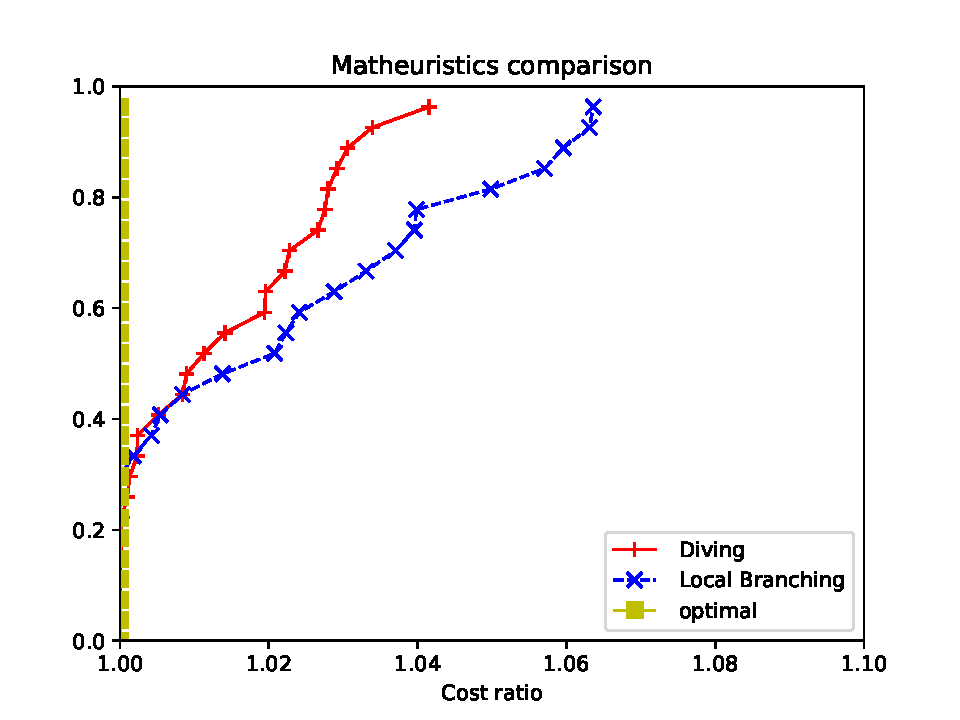
\includegraphics[width=0.7\linewidth]{Immagini/math.pdf}
    \caption{Performance profile of all Matheuristic methods.}
    \label{fig:math_comp}
\end{figure}
    \chapter{Conclusions}

\section{Performance Profile plots}
The Performance Profiler \cite{dolan2002benchmarking} is a tool that facilitates the visualization of comparisons between the results of different algorithms. Depending on the type of algorithm, users can choose to compare various aspects of the results. In our case, when comparing heuristic methods, we are interested in the quality of the solutions found, so we use the solution cost as the metric. Conversely, when comparing exact algorithms, the solutions are always the same (the optimal one), but the focus shifts to the time required to find these solutions.

The performance profile classifies the execution times (or solution costs) based on the success percentage relative to a multiplication factor (ratio). The trend of the performance profile of an algorithm is monotonically increasing. The value for each ratio in the graph represents the percentage of instances that the algorithm solves with that factor compared to the optimum for that case. These graphs are often represented on a logarithmic scale to better highlight differences and achieve a clearer depiction.

The program used to create the performance profiles of the different algorithms is \textit{perprof.py}, developed by D. Salvagnin in 2016 \cite{salvagnin2016performance}.

\section{Heuristic and Metaheuristic methods}
The diagram illustrates the performance of various heuristic and metaheuristic methods for solving the Traveling Salesman Problem (TSP): Nearest Neighbor (NN), NN with 2-opt optimization, NN with Tabu Search, and NN with Variable Neighborhood Search (VNS). The Nearest Neighbor (NN) method is the least effective, with solutions deviating 15-20\% from the optimal cost, as shown by the red curve. Applying 2-opt optimization significantly improves the NN method, achieving solutions within 5\% of the optimal cost, indicated by the blue curve. Both Tabu Search and VNS perform similarly, with solutions within approximately 5\% of the optimal cost, as shown by their overlapping green and purple curves. The 2-opt method alone can nearly match the performance of Tabu Search and VNS, demonstrating its effectiveness. All enhanced methods perform significantly better than the basic NN method, highlighting the importance of optimization techniques in solving the TSP.

The performance profile in Figure \ref{fig:heur_comp} shows that while NN is quick, its performance is suboptimal. Incorporating optimization techniques like 2-opt, Tabu Search, or VNS improves solution quality, reducing the error margin to within 5\% of the optimal solution. The similar performance of 2-opt, Tabu Search, and VNS suggests that the choice among them can be based on computational efficiency or implementation complexity rather than solution quality. This analysis highlights the critical role of optimization in heuristic approaches to combinatorial problems like the TSP.

\begin{figure}[H]
    \centering
    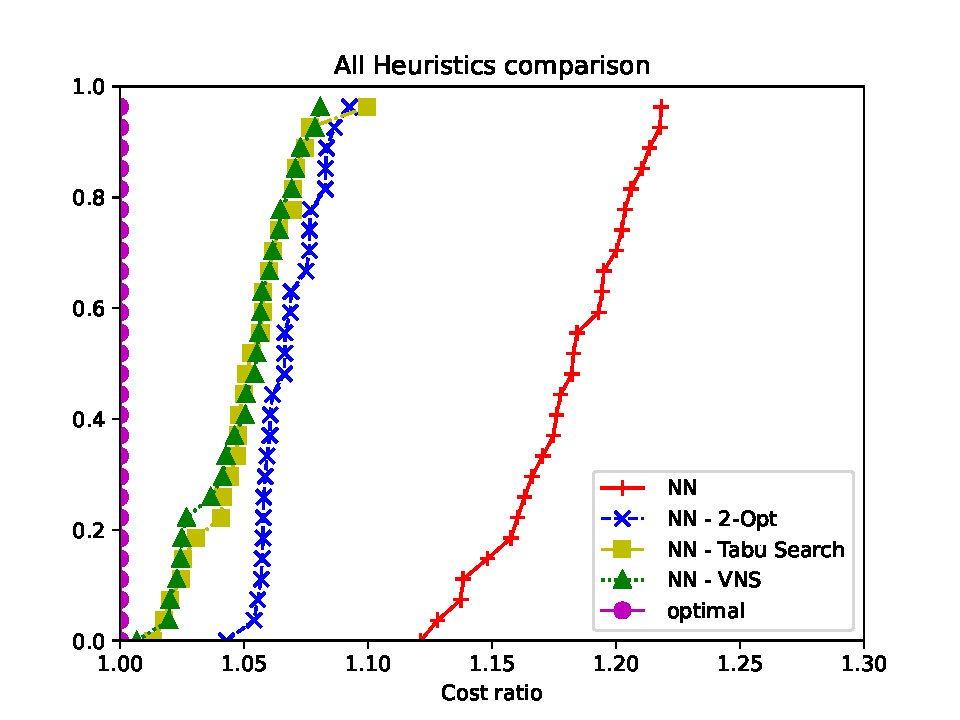
\includegraphics[width=0.7\linewidth]{Immagini/All Heuristics.pdf}
    \caption{Performance profile of all Heuristics methods.}
    \label{fig:heur_comp}
\end{figure}

\section{Exact Methods}
The diagram in Figure \ref{fig:exacts_comp} compares the performance profiles of various exact methods for solving optimization problems, focusing on Benders' decomposition and Branch-and-Cut (B\&C) techniques with different enhancements. Utilizing all available features, such as MIP Start, candidate callback, user-cut callback, and posting, yields the best performance, significantly improving efficiency and solution quality. Even using only the posting method the performance remains highly effective, indicating that it is a particularly powerful technique. The plain B\&C approach with callbacks is effective as much as Benders' loop method, indicating that with our modern computational power even a simpler method can reach very good results.

Overall, the analysis demonstrates that while both Benders' decomposition and B\&C methods are powerful, the strategic use of enhancements like callbacks, MIP start and especially posting significantly influences their performance, making them more efficient and adaptable to real-world scenarios.

\begin{figure}[H]
    \centering
    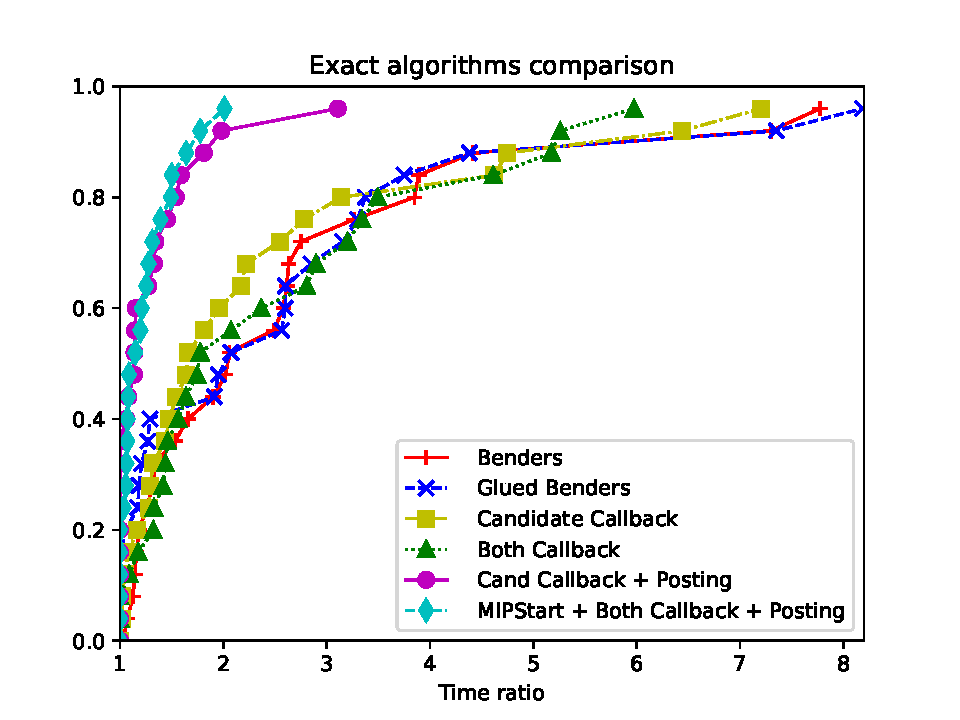
\includegraphics[width=0.7\linewidth]{Immagini/exacts.pdf}
    \caption{Performance profile of all Exact methods.}
    \label{fig:exacts_comp}
\end{figure}

\section{All Heuristics and Matheuristics Methods}
From the results presented in the performance profile in Figure \ref{fig:allheur_comp}, it is evident that matheuristic algorithms significantly outperform both heuristic and metaheuristic algorithms. Within the same category of algorithms, performance differences are almost negligible, except for the Nearest Neighbor (NN) algorithm, which stands out as the least performing among all the considered algorithms. The application of VNS and Tabu Search significantly improves the performance of the Nearest Neighbor algorithm, although the results obtained still do not reach those of Local Branching, which clearly stands out for its better performance. However, Local Branching is consistently outperformed by the Diving algorithm, who seems to be the best one among all the non-exact algorithms.

\begin{figure}[H]
    \centering
    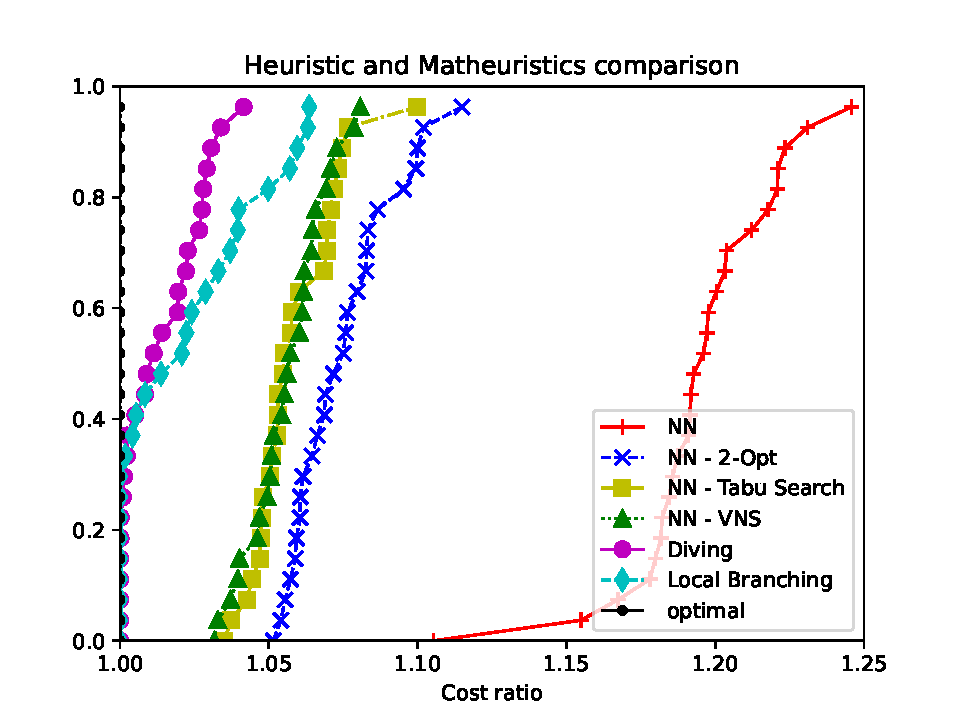
\includegraphics[width=0.7\linewidth]{Immagini/all_heur.pdf}
    \caption{Performance profile of all Heuristic and Matheuristic methods.}
    \label{fig:allheur_comp}
\end{figure}

\section{Final Conclusions}
In conclusion, we can affirm that each algorithm has unique characteristics that make it suitable for specific scenarios and objectives. The choice of the most appropriate algorithm depends on the specific needs of the problem to be solved and the available resources.

If the main goal is to obtain a solution in a short time, even at the cost of not necessarily achieving optimality, heuristic, metaheuristic, and matheuristic algorithms are a valid choice. These approaches use approximation strategies and advanced search techniques to find good solutions quickly, making them ideal for complex problems where speed is essential.

On the other hand, if the aim is to obtain a solution that is as close as possible to the optimum, without considering computation time as a critical factor, exact algorithms are the best choice. These algorithms are designed to explore the entire solution space, thus ensuring the possibility of finding the optimal solution or the one closest to the optimum, albeit at the cost of longer computation times.

In summary, the selection of the algorithm depends on the need to balance solution quality and execution time. Understanding the characteristics and capabilities of each type of algorithm allows for informed decisions and optimization of resources to achieve the desired results in the most efficient way possible.

    \clearpage

    \printbibliography[heading=bibintoc]
\end{document}
